\chapter{Background subtraction}
\section{Assessing Beamline Contamination}
Even if pions are by far the biggest beam component in negative polarity runs, the LArIAT beam is not a pure pion beam. While useful to discriminate between pions, kaons, and protons, the beamline detectors are not sensitive enough to  discriminate among the lighter particles in the beam: electrons, muons and pions fall under the same mass hypothesis. Thus, we need to assess the contamination from beamline particles other than pions in the event selections used for the pion cross section analysis and correct for its effects.


We define beamline contamination every TPC track matched to the WC track which is not a primary pion. Potentially, there are 4 different types of beamline contaminations:
\begin{itemize}
\item[]1) electrons,
\item[]2) muons,
\item[]3) secondaries from pion events,
\item[]4) matched pile up events.
\end{itemize}

So, how do we handle this contamination?
The first step is to estimate what percentage of events used in the cross section calculation is not a primary pion.  The next two sections will illustrate this estimate for the electrons, muons and secondaries from pion event.
We estimate the last type of contamination, the ``matched pile up" events, to be a negligible fraction, because of the definition of the WC2TPC match: we deem the probability of a single match with a halo particle in the absence of a beamline particle\footnote{ Events with multiple WC2TPC matches are always rejected.} negligibly small.


\subsection{Electron and Muon contamination}
We estimate the percentage of electrons and muons in the beam via the beamline MC. 
Since the beamline composition is a function of the magnet settings, we simulate separately events for magnet current of -60A and -100A. 

\begin{figure}
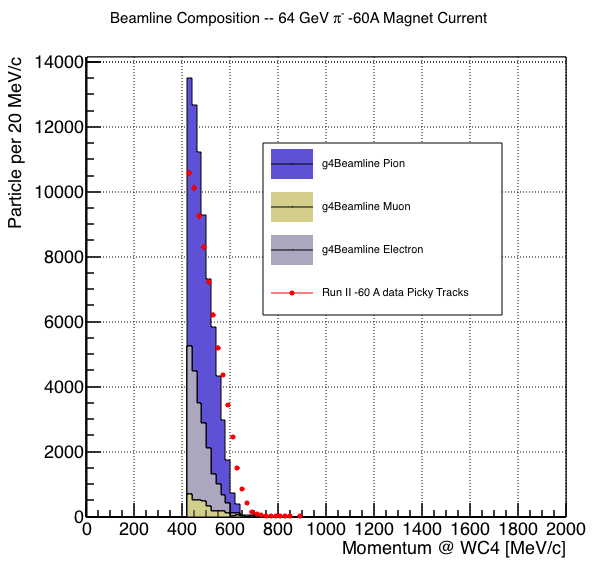
\includegraphics[width=0.5\textwidth,height=\textheight,keepaspectratio]{Chapter-7/Images/Beam60A.png}
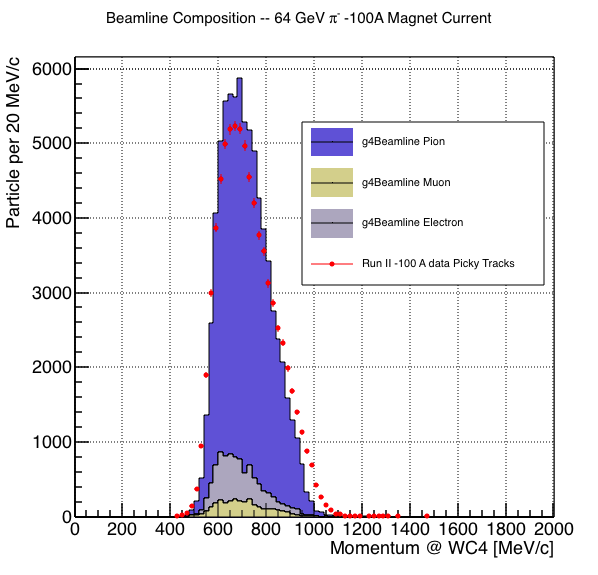
\includegraphics[width=0.5\textwidth,height=\textheight,keepaspectratio]{Chapter-7/Images/Beam100A.png}
\caption{Beam composition for the -60A runs (left) and -100A runs (right). The solid blue plot represents the simulated pion content, the yellow plot represents the simulated muon content and the grey plot represents the simulated electron content. The plots are area normalized to the number of data events, shown in red. }
\label{fig:BeamComposition}
\end{figure}

Table \ref{tab:beamline} shows the beam composition per magnet setting after the mass selection according to the G4Beamline simulation.
\begin{table}[]
\centering
\begin{tabular}{|l|c|c|}
\hline
                     & I = -60 A           & I = -100 A \\ \hline
G4Pions       &   68.8 \%           &      87.4 \%        \\ \hline
G4Muons     &     4.6 \%           &        3.7 \%         \\ \hline
G4Electrons &   26.6 \%           &        8.9 \%        \\ \hline
\end{tabular}
\caption{Simulated beamline composition per magnet settings}
\label{tab:beamline}
\end{table}


\begin{table}[]
\centering
\begin{tabular}{|l|c|c|c|c|c|}
\hline
                                                     & I = -60 A          & I = -100 A   & Total     &  w$_{60A}$ &  w$_{100A}$\\ \hline
N Data Events after Mass Selection     &     70192          &  76056       & 146248 & 0.48 & 0.52\\ \hline
%Data events for Cross Section          &                         &                   &              & & \\ \hline
%Estimated e in the beamline             &   18671.1         &    6769.0  &              & & \\ \hline
%Estimated $\mu$ in the beamline     &     3228.8         &     2814.1     &              & & \\ \hline
%Estimated $\pi$ in the beamline       &    48292.1        &   66472.9   &              & & \\ \hline
\end{tabular}
\caption{Number of data events which fit the pion mass hypothesis as a function of magnet settings. The last two columns represent the faction of the data in the given magnet setting.}
\label{tab:databreakdown}
\end{table}



We calculate the electron to pion, as well as the muon to pion ratio on the whole sample as the weighted sum of the corresponding ratio in the two current settings, 
\begin{equation}
\frac{N_e}{N_\pi}_{Data} = w_{60A}\frac{N_e}{N_\pi}_{60A}  + w_{100A}\frac{N_e}{N_\pi}_{100A},
\end{equation}
\begin{equation}
\frac{N_\mu}{N_\pi}_{Data} = w_{60A}\frac{N_\mu}{N_\pi}_{60A}  + w_{100A}\frac{N_\mu}{N_\pi}_{100A},
\end{equation}
where the weights $w_{60A}$ and $w_{100A}$ are the percentage of events in the corresponding magnet configuration passing the mass selection in data, as shown in table \ref{tab:databreakdown}. Figure \ref{fig:BeamComposition} shows the mometum predictions from G4Beamline overlaid with data for the 60A runs (left) and for the 100A runs (right). The predictions for electrons, muons and pions have been staggered and their sum is area normalized to data. Albeit not perfect, these plots show a reasonable agreement between the momentum shapes in data and MC. We attribute  the difference in shape to the lack of simulation of the WC efficiency in the MC which is momentum dependent and leads to enhance the number events in the center of the momentum distribution.


Once the beam composition is know,  we simulate the electrons, muons and pions with the DDMC and we subject the three samples to the same selection chain (WC2TPC match, shower filter, pile up filter). The percentage of electrons and muons surviving the selection chain weighted by the beam composition is the  electron and muon contamination in the pion cross section sample, as shown in Table \ref{tab:MCafterCutContaminants}.

\subsection{Contamination from secondaries}
Pions can travel the length of the LArIAT beamline and interact hadronically in the steel or in the non-instrumented argon upstream to the TPC front face.  One of these products can leak into the TPC and be matched with the WC track, contribuiting to the pool of events used for the cross section calculation. We call this type of particles ``secondaries" from pion events, with a terminology inspired by Geant4. 
We estimate the number of secondaries using the DDMC pion sample.  The percentage of secondaries is given by the number of matched WC2TPC tracks whose corresponding particle is not flagged as primary by Geant4 and is not a muon, to avoid double counting with the G4Beamline estimate.  The secondary to pion ratio is $X$\% in the 60A sample and $Y$\% in the 100A sample.

\section{Beamline Background Subtraction}
Once we estimate the contaminants to primary pion ratio, the next step is subtracting their collective contribution from data. To do so, we simulate the same number of electrons, muons and pions with the DDMC separately for the two magnet settings, and we apply the same selection filters on the three samples. The number of events per particle species surviving this selection is shown on table \ref{tab:MCafterCutContaminants}.

\begin{table}[]
\centering
\begin{tabular}{| l | l | l | l | l | l | l | l | }
\hline
                                                  &  $\pi^-$  60A  & $\mu^-$ 60A & $e^-$  60A & $\pi^-$ 100A  & $\mu^-$ 100A & $e^-$  100A  \\
\hline
Total Initial events ��                  & 334500   & 334500  & 334500  & & & \\
After Multiplicity Rejection & 331313   & 322436   &  186261& & &\\
After WC2TPC: Selection &�201458   &  285686  &  79109  & & & \\
Evts After Shower Rejection ���& 191655   &  277914 &  17477    & & &\\
  \hline
  ���&     &   &     & & &\\
Survival rate               &57\%��&  83\%   & 5\%  &     &  &\\
  ���&     &   &     & & &\\
Beam Composition               &     &   &     & & &\\ 
After Selection   ���                &     &   &     & & &\\
  ���                                        & 88.5\%  & 8.5\%  &  3\%   & & &\\
\hline
%         &                              &             &                      &  \\ \hline
\end{tabular}
\caption{MC selection flow per particle species.}
\label{tab:MCafterCutContaminants}
\end{table}


\begin{figure}[h!]
\centering
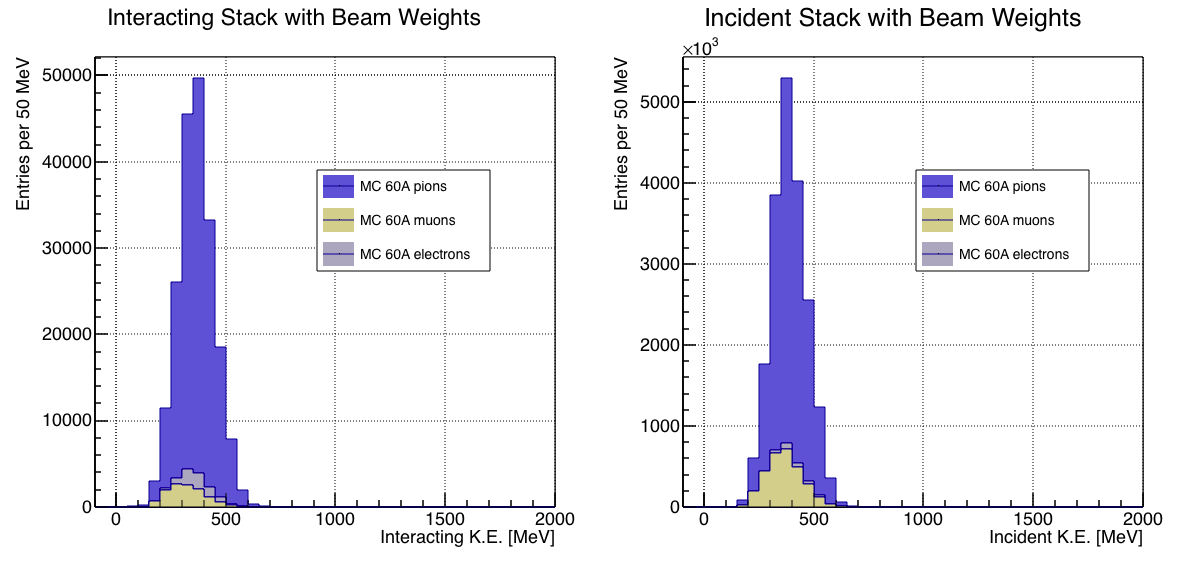
\includegraphics[width=\textwidth]{Chapter-7/Images/Staggered60A.png}
\caption{Left: staggered contributions to the interacting kinetic energy distribution for electron (grey), muons (yellow) and pion (blue) in the 60A simulation sample. Right: staggered contributions to the incident kinetic energy distribution for electron (grey), muons (yellow) and pion (blue) in the 60A simulation sample.  }
\label{fig:stag60A}
\end{figure}



We then produce the interacting and incident histograms for the events surviving the selection for both the pions and the contaminants, weighted by the estimated beam composition.


\begin{figure}
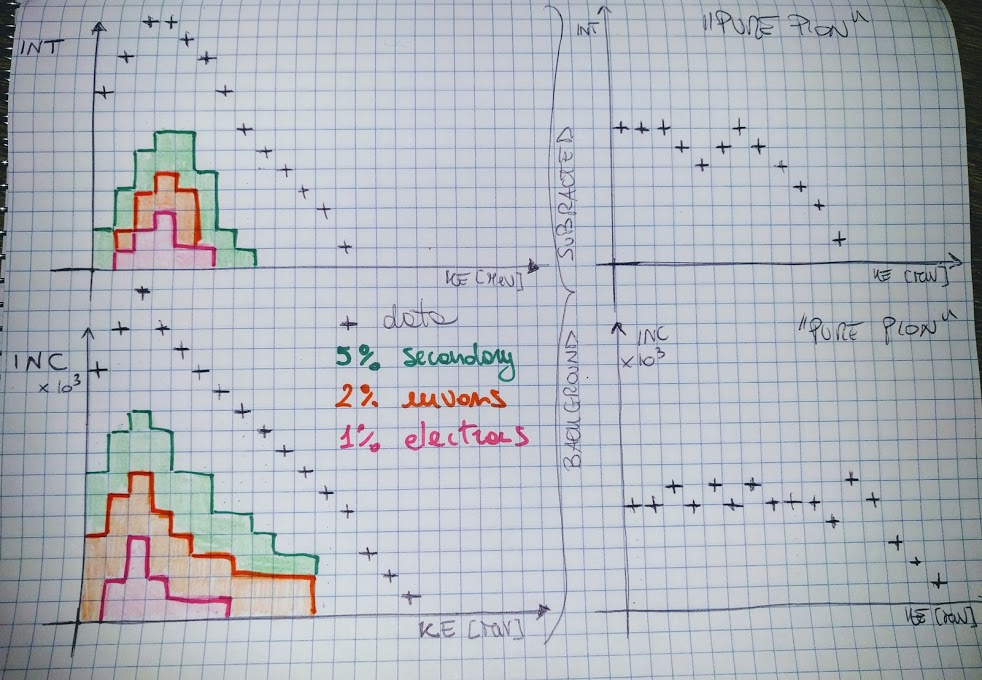
\includegraphics[width=\textwidth,height=\textheight,keepaspectratio]{Chapter-9/Images/FakePlot.jpg}
\label{fig:backgroundSubtraction}
\caption{A graphical rendering of the beamline contamination background subtraction. The contribution of the contaminants is shown in green for the secondaries, in orange for the muons and in pink for electrons. The colored plots are coming from the MC and are staggered. The percentages shown in the legend are the percentages of contaminants over the total number of events  passing the selection chain. We actually expect way less contamination.}
\end{figure}

We then evaluate the relative contribution of the contaminants bin by bin in the interacting and incident histograms separately. In data, we subtract this estimated relative contaminants contribution on the interacting and incident histograms  bin by bin.


We estimate the systematic uncertainty on the cross section from this subtraction procedure by varying the electron to pion and muon to pion ratio in a suitable range of values. Figure  


\section{Capture and decay}\label{ch:CaptureAndDecay}
Our goal is to measure the total hadronic cross section for negative pions in argon. Since pion capture can be classified as an electromagnetic process and pion decay is a week process,  capture and decay represent unwanted interactions. We present here a study of capture and decay in Monte Carlo and the solution we adopted to mitigate their present in the data sample. 

For this MC study, we use a sample of 359000 MC pions generated according to the beam profile with the DDMC described in \ref{sec:DDMC}. It is important to notice that capture occurs predominantly at rest, while decay may occur both in flight and at rest. Thus, we can highly mitigate capture and decay at rest by removing pions which would release all their energy in the TPC and stop. This translates into a momentum selection, where we keep only events whose WC momentum is above a certain threshold. 
Figure \ref{fig:CaptureMom} shows the true momentum distribution for the primary\footnote{We use here the Geant4 denomination ``primary" to indicate that the pion considered does not undergo interactions modifying its energy before getting to the TPC. In fact, not every pion shot from wire chamber four will arrive to the TPC as primary,  some will decay or interact before the TPC.} pions that arrive to the TPC (pink), that capture (green) or decay (blue) inside the TPC, on a linear and log scale vertical axis. 

\begin{figure}[hpbt]
\centering
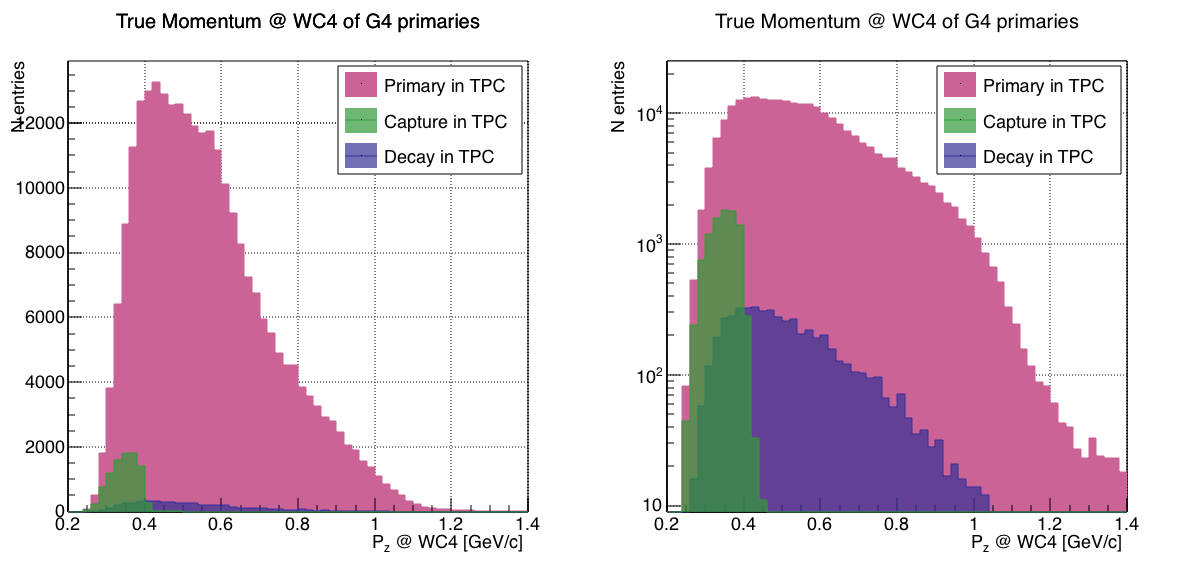
\includegraphics[width=15cm]{Chapter-7/Images/CDAsMomentumFunct.png}
\caption{True momentum distribution at wire chamber 4 for every simulated pion arriving in the TPC (pink), ending its life in capture (green) or in decay (blue) in the TPC, linear vertical axis on the left, logarithmic on the right. }
\label{fig:CaptureMom}
\end{figure}


In order to choose the selection value for the wire chamber momentum, it is beneficial to estimate the ratio of events which capture or decay that survive the selection in MC as a function of the momentum threshold, and compare it with the survival ratio for all events. This is done in figure \ref{fig:survRatio}. We define the survival ratio simply  as the number of events surviving the true momentum selection divided by the number of events of that category. We calculate the survival ratio separately for the three event categories explained above: total (pink), capture (green) and decay (blue).
Selecting pions with momentum greater than 420 MeV/c reduces the capture events by ~99\% while maintaining about 80\% of the total data sample. 
Figure \ref{fig:evtRatio} shows the ratio of events which end their life in capture (green) or decay (blue) over the total number of events as a as a function of the true momentum at wire chamber four. This ratio is slightly dependent on the inelastic cross section implemented in Geant4, as we are able to register a pion capture (or decay) only if it did not interact inelastically in the TPC. We choose a momentum threshold of 420~MeV/c because the percentage of capture events drops below 1\% and the percentage of decays is never above 2\% for momenta greater than 420~MeV/c.

\begin{figure}[h!]
\centering
\begin{minipage}[t]{0.45\textwidth}
\centering
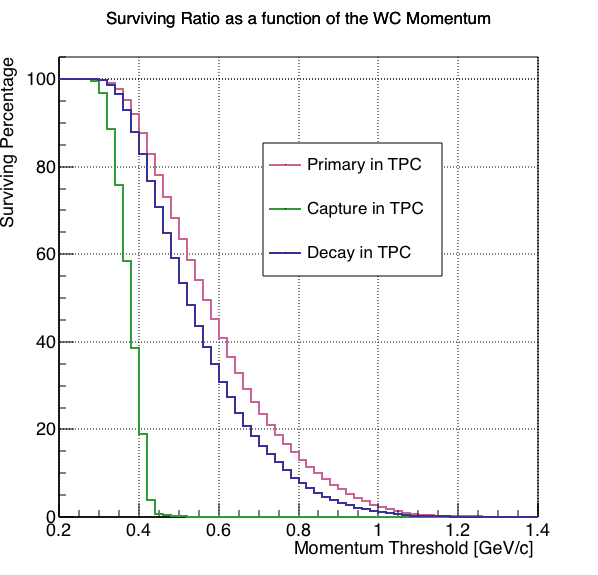
\includegraphics[width=7.5cm]{Chapter-7/Images/CDThreshold.png}
\caption{Survival ratio as a function of selection threshold on true momentum at wire chamber four for for every simulated pion arriving in the TPC (pink), capture (green) or in decay (blue).   }
\label{fig:survRatio}
\end{minipage}\hfill
\begin{minipage}[t]{0.45\textwidth}
\centering
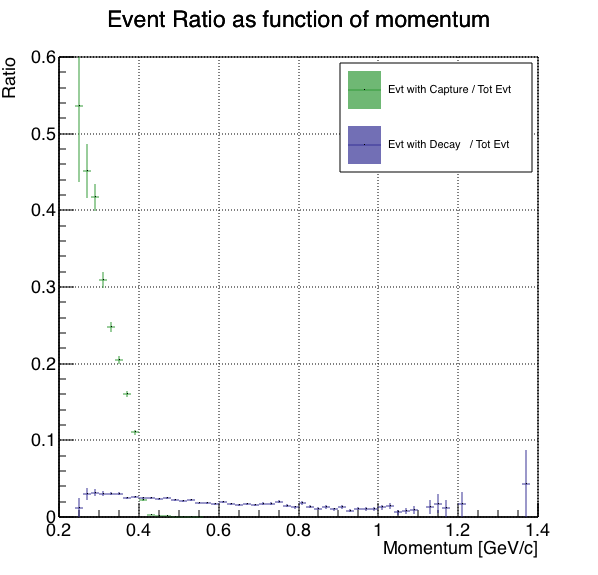
\includegraphics[width=7.5cm]{Chapter-7/Images/CDRatio.png}
\caption{Ratio between the capture (green) and decay (blue) events over the total number of events as a as a function of the true momentum at wire chamber four.}
\label{fig:evtRatio}
\end{minipage}
\end{figure}


